\subsection{Experimental program}
The study is organized as two empirical tiers over three claim axes, summarized in
Figure~\ref{fig:program}. A black-box tier (Tier~1) characterizes a frontier model
behaviourally as the resilient reference end; a white-box tier (Tier~2) performs
mechanistic interpretability on open weights, where the residual stream is directly
observable and editable. Both tiers feed three distinct claim axes---mechanism
(Axis~A: refusal direction, EC50, dimension), functional analogy (Axis~B: order
parameter, monitoring precision), and metaphor with a falsifiable core (Axis~C:
avasth\=atraya and the \d{s}a\d{t}karma)---and a cross-axis triangulation then tests,
on the same prompts, whether internal monitor collapse predicts behavioural capture.

\begin{figure}[h]
\centering
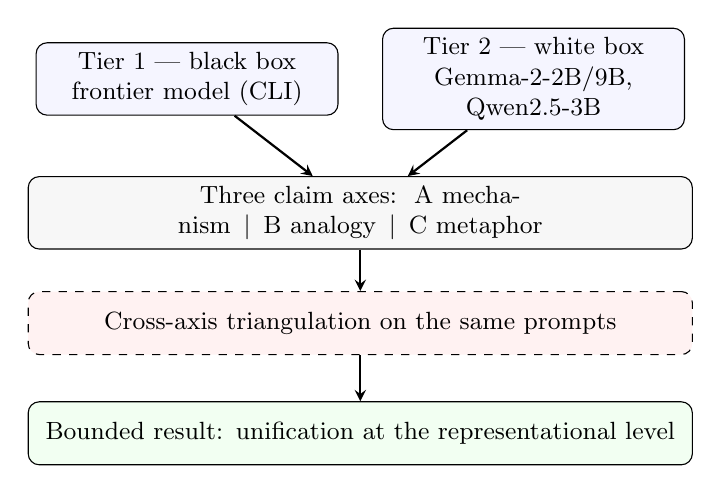
\begin{tikzpicture}[
  font=\small,
  b/.style={rectangle, draw, rounded corners, align=center, minimum height=0.85cm,
    text width=3.6cm, fill=blue!4},
  ax/.style={rectangle, draw, rounded corners, align=center, minimum height=0.8cm,
    text width=8.2cm, fill=gray!6},
  key/.style={rectangle, draw, rounded corners, dashed, align=center,
    minimum height=0.8cm, text width=8.2cm, fill=red!5},
  res/.style={rectangle, draw, rounded corners, align=center, minimum height=0.8cm,
    text width=8.2cm, fill=green!5},
  a/.style={thick, -stealth}
]
\node[b] (t1) at (-2.2,0) {Tier 1 --- black box\\frontier model (CLI)};
\node[b] (t2) at (2.2,0) {Tier 2 --- white box\\Gemma-2-2B/9B, Qwen2.5-3B};
\node[ax]  (ax) at (0,-1.7) {Three claim axes:\, A mechanism \,\textbar\, B analogy \,\textbar\, C metaphor};
\node[key] (tr) at (0,-3.1) {Cross-axis triangulation on the same prompts};
\node[res] (rs) at (0,-4.5) {Bounded result: unification at the representational level};
\draw[a] (t1) -- (ax);
\draw[a] (t2) -- (ax);
\draw[a] (ax) -- (tr);
\draw[a] (tr) -- (rs);
\end{tikzpicture}
\caption{The two-tier, three-axis program in which both tiers feed three claim axes
and a cross-axis triangulation bounds the unification.}
\label{fig:program}
\end{figure}

\subsection{Models and substrate}
The white-box tier studies three instruction-tuned open-weight chat
models---Gemma-2-2B-it (26 layers, $d=2304$), Gemma-2-9B-it (42 layers,
$d=3584$), and Qwen2.5-3B-Instruct (36 layers, $d=2048$)---on a single NVIDIA GB10
(Grace--Blackwell) accelerator. The black-box tier probes a frontier model (Claude)
behaviourally through its command-line interface. All white-box interventions are
implemented as PyTorch forward hooks on the decoder layers and the token embedding;
higher-level interpretability wrappers are deliberately avoided to retain exact
control over the residual stream.

\subsection{Refusal direction and interventions}
Let $h^{(\ell)}(x)\in\mathbb{R}^d$ be the residual stream at the last prompt token
of layer $\ell$ for input $x$. Given matched harmful prompts $\mathcal{H}$ and
harmless prompts $\mathcal{S}$, the difference-in-means direction is
\begin{equation}
\mathbf{d}^{(\ell)} = \frac{1}{|\mathcal{H}|}\sum_{x\in\mathcal{H}} h^{(\ell)}(x)
- \frac{1}{|\mathcal{S}|}\sum_{x\in\mathcal{S}} h^{(\ell)}(x),
\qquad \dref = \mathbf{d}^{(\ell)}/\norm{\mathbf{d}^{(\ell)}}.
\end{equation}
Directional ablation removes $\dref$ from every write to the residual
stream (embedding and all layer outputs), scaled by $\alpha\in[0,1]$:
$h \mapsto h - \alpha (h\cdot\dref)\dref$. Activation addition adds
$c\,\dref$ at the extraction layer. For multi-direction (subspace) ablation a
matrix $D$ is orthonormalized (QR) and its span removed. The extraction layer is
selected on a held-out validation split disjoint from the evaluation split.

\subsection{Outcome measures}
Refusal is detected with an Arditi-style substring metric over the opening span of
the generation; attack success rate (ASR) is the fraction of harmful prompts that
comply, and over-refusal is the fraction of harmless prompts that refuse.
Because automatic refusal metrics can be biased (Section~\ref{sec:results}), the
primary behavioural claims are additionally validated by a content-faithful
LLM-judge and by manual inspection. Pure-text measures support the
\d{s}a\d{t}karma acts: degeneracy ($1-$ mean unique-token ratio), answer divergence
($1-$ Jaccard token overlap between paired generations), and coherence (mean
unique-token ratio of non-empty outputs).

\subsection{Dose--response and dimensionality}
The dose--response sweeps $\alpha$ and fits a four-parameter logistic
$\mathrm{ASR}(\alpha)=l+(h-l)/(1+e^{-k(\alpha-\alpha_{50})})$, reporting EC50
$=\alpha_{50}$. The refusal-subspace effective dimension is measured by iterative
logistic projection: a probe is fit to separate $\mathcal{H}$ from $\mathcal{S}$,
its cross-validated accuracy is recorded, the probe direction is projected out of
the activations, and the procedure repeats; the effective dimension is the number
of directions whose removal drives accuracy to chance. This dimension is computed
at the extraction layer and, to test its stability, at every layer.

\subsection{The symmetry order parameter}
The refusal order parameter for an activation is the normalized projection
$m(h) = (h\cdot\dref)/\norm{h}$. For a request $r$, a paraphrase orbit
$\mathcal{O}(r)$ of meaning-preserving rephrasings is formed and $m$ is measured
across the orbit. The invariance of refusal under the rephrase group action is
quantified by the between-class to within-orbit variance ratio (an $F$-ratio) of
$m$, compared against a random-direction control. Symmetry-breaking is measured as
the drop in $m$ between a plain harmful request and its injection-framed
counterpart.

\subsection{The \d{s}a\d{t}karma as interventions}
Each of the six acts is operationalized as a distinct activation intervention with
a matched control: vaś\=\i kara\d{n}a (ablate $\dref$, measure ASR), ś\=anti (add
$\dref$, measure over-refusal), stambhana (ablate the dominant residual principal
component, measure degeneracy), vidve\d{s}a\d{n}a (steer a factual answer off
baseline, measure divergence), ucc\=a\d{t}ana (ablate a category-specific
direction, measure selective ASR), and m\=ara\d{n}a (ablate the top-$k$ principal
components or, in a stronger variant, the top-$K$ most-active sparse-autoencoder
features, measuring coherence collapse). An act is judged ``control-separated'' if
its effect exceeds its matched control by a fixed margin.

\subsection{Statistics, controls, and pre-registration}
All gates use bootstrap confidence intervals and, for probes, a label-shuffled
null and a layer-0 (surface) baseline; ablation effects are checked against
multiple ($\geq 10$) random-direction controls. Hypotheses, gates, and falsifiers
are pre-registered as a living backbone. Every metaphysical-tier claim must pass a
transfer gate (held-out prompts), a null gate (better than shuffled
labels), and a surface gate (better than a layer-0 baseline) before it is
retained; failure triggers a documented demotion rather than a silent drop.
